\chapter{Technical Issues}\label{chapter:technicalissues}
This chapter covers some of the problems encountered when turning the model from Chapter \ref{chapter:model} into code. This will not be an exhaustive list of all the challenges but will focus on the more interesting problems and solutions.

  \section{ABM frameworks}
    \paragraph{What is an ABM framework?}
    The first challenge was to create a software environment to run the simulation. 
    \paragraph{Why use an ABM framework? - Gilbert and Bankes paper}
    Gilbert and Bankes (\cite{Gilbert2002}) explain the advantages and
    disadvantages of using pre-existing libraries and frameworks for Agent-Based Models rather
    than ``rolling your own.'' Using pre-existing libraries frees a
    programmer up from re-implementing common
    algorithms. However, they also require a programmer to understand the
    language they are written in and to work with the built-in
    assumptions used by the original writers. Gilbert and Bankes state
    that agent-based modeling tools that match their ideal specifications
    do not yet exist but that there is a trend towards better
    tools becoming available. Fortunately a few years later Allen (\cite{Allan2009}) and Berryman (\cite{Berryman2008}) survey many ABM frameworks and suggest that NetLogo, MASON and Repast are useful frameworks. Personal communication with EngD student Ed Manley (\cite{Manley2012}) at UCL working on traffic simulations led me to look at the Repast framework. Therefore it seemed in 2012 with only a few months to complete this project but a good understanding of Java, using a pre-built framework would require less work than starting from the bottom and building a framework dedicated to the project.
    \subsection{ABM frameworks considered}
      \paragraph{Review of ABM frameworks - Allen and Berryman papers, hands}
      \subsubsection{Repast}
        \paragraph{descriptions of features/pros and cons of Repast}
        Open source
        Mailing list
        Documentation
        Examples from Repast City
        Java
        Random number generation
        Integrates nicely with Eclipse (so quick to get started)
        - slower than mason
        - less support for learning algorithms
      \subsubsection{NetLogo}
        \paragraph{descriptions of features/pros and cons of Netlogo}
        NetLogo requires the use of a proprietary
        language to program the agents aimed at beginner programmers, which I
        found too restrictive.
        Does not require much programming experience
        
      \subsubsection{MASON}
        Similar to RePast (in fact grew out of RePast according to )
    \subsection{The ABM framework I used}
      \paragraph{Why I chose ABM}
      Personal recommendation and one-to-one tutorial with a user. Berryman finds little to separate MASON and RePast so this is enough to swing it.
      Don't need to be able to handle a large number of agents (1000 boats fill the river)
      
  \section{Building the river}
    The river presented two challenges. Even with the decision to represent it in the model as three graphs to represent the three lanes there was still the challenge of determining the value of the location attribute for each node. Then there was the problem of drawing this river in the visualization.
    
    \subsection{Rastorization vs vectorization}
    
      \paragraph{Storing river as a series of squares/pixels}
      Early models of the river had it as an open space in which a boat was free to move. Therefore it seemed easier to store the river for visualization as a series of squares (effectively pixels). This made collision detection with the bank easier (only had to check that the whole boat was on the finite number of river squares). Unfortunately it was not easy to represent this easily in Repast. Although it had the ability to draw the grid and keep track of which were river squares and which were not. However, it could not do this in an efficient manner and would recalculate the value of the square at each tick. Also it was difficult to draw smooth corners.
      
      \paragraph{Storing river as a series of vectors (or nodes separated by vectors)}
      \paragraph{Breaking down river into 1D lanes adds benefits to vectorization}
      The solution came with the idea to treat the river as 3 lanes. Each lane is then drawn using series of vectors between each node. Since the length of each vector is fixed at 20m, it was just a case of storing the angle from one node to the next. To get the form a 2D outline of each lane as well as storing the location of the node in the graph, the location of a point 5m to each side of the node was stored. These three locations were determined by taking the three points (20, 5), (20, 0) and (20, -5) and rotating them by the angle associated with the next vector and then translating them by the location of the last placed node. The outline of the river of was then formed by using the top boundary of the top lane and the bottom boundary of the bottom lane. It was then easy in Java using the Path2D.Double class to form this arbitrary shape which RePast was then able to display.
      
      The next challenge was to work out the angle of each vector. This was done using Google Earth to create a simplified version of the river Cam. Though the technique would work for any shape of river that was three lanes wide.
      
      Any any parts of the river that were nearly straight were treated as being fully straight. It was then just a case of using the ruler tool in Google Earth to work out how many 20m straight lines would make up each straight. At the start of the section of the Cam this project covers the river nearly heads roughly East (or alternatively the river has been rotated so that it appears to head directly right on the screen). For simplicity it was considered to be heading due East, so the angle of the first few vectors was 0 and the river was started at (0,10), (0,20), (0,30) for the nodes of the three lanes. See \ref{fig:thereach} for a screen shot of Google Earth of this first section of river.
      
      \begin{figure}[H]
      \begin{center}
      	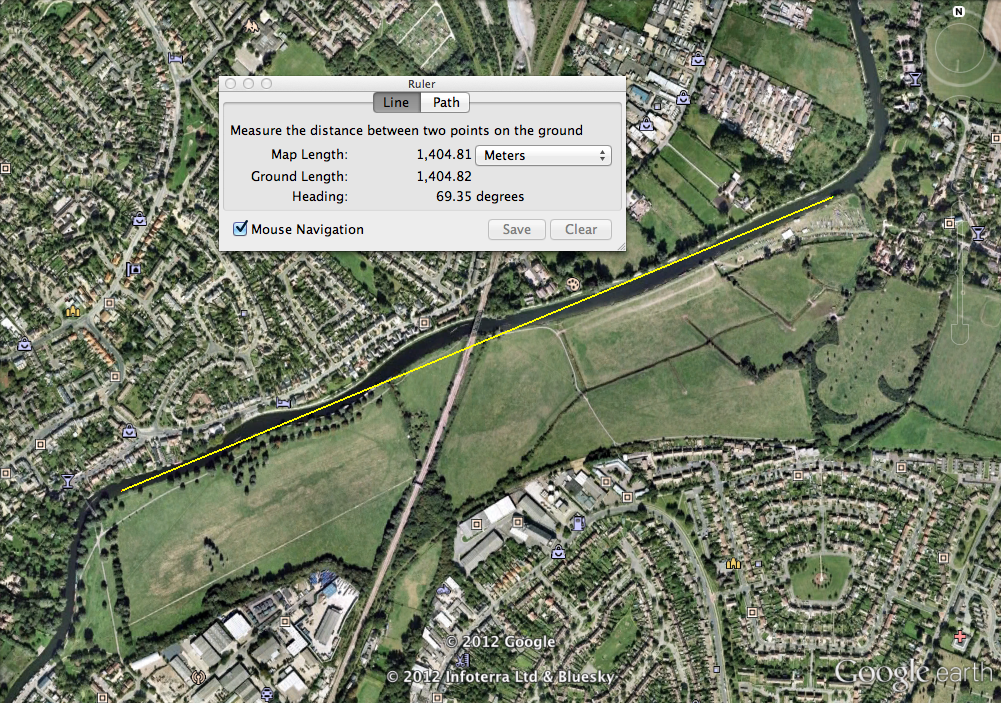
\includegraphics[scale=0.3]{images/TheReach.png}
      	\caption{The Reach: roughly 1400m long and straight. By rotating the whole river 20\textdegree \ clockwise can treat it as 70 lots of 20m vectors heading having an angle of 0\textdegree \ from the horizontal (the line apporoximation in Google Earth has a heading of 70\textdegree but this is a bearing so measured clockwise from North unlike standard geometry which measures anti-clockwise from the $x$-axis.)}
      	\label{fig:thereach}
      \end{center}
      \end{figure}
      
      Corners were then approximated using sectors a circle, with the river following the arc of the sector. Using Google Earth the radius of the circle of curvature was estimated very approximately. The angle of the sector was approximated by looking at the bearing of line heading into the corner and the bearing of a line heading out of the corner. The angle of the sector was then the difference of these two bearings.
      
      \begin{figure}[H]
      \begin{center}
      	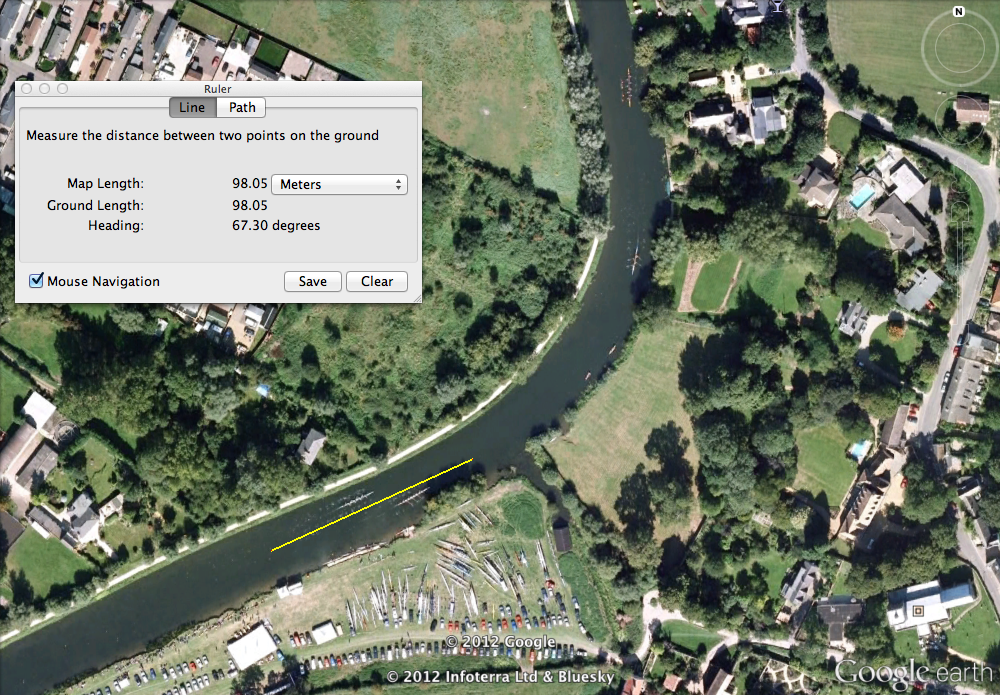
\includegraphics[scale=0.3]{images/DittonCornerHeadingIn.png}
      	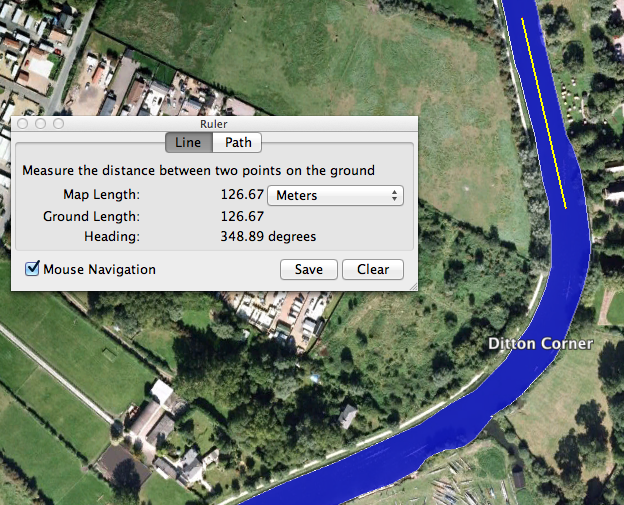
\includegraphics[scale=0.3]{images/DittonCornerHeadingOut.png}
      	\caption{Ditton Corner: The heading in is roughly 70\textdegree and the heading out is roughly 170\textdegree so treated this corner as a 90\textdegree sector of a circle (by using a right-angle the calculations were a bit simpler).}
      	\label{fig:dittoncorner:angle}
      \end{center}
      \end{figure}
      
      \begin{figure}[H]
      \begin{center}
      	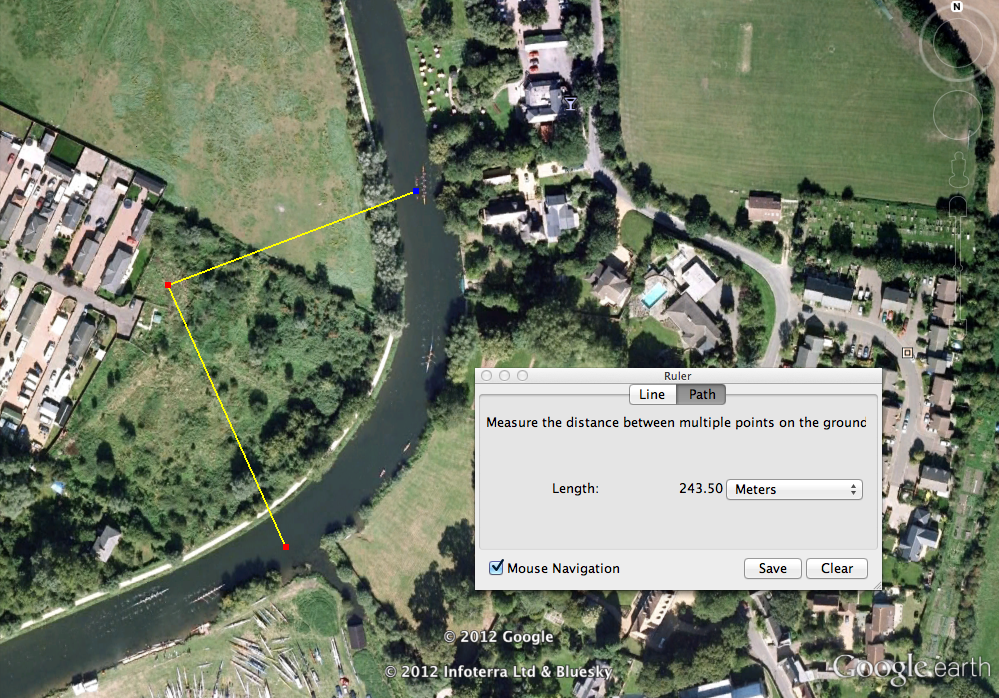
\includegraphics[scale=0.3]{images/DittonCornerRadius.png}
      	\caption{Ditton Corner: This shows two approximate radii of the sector that makes up Ditton Corner. Their total length is 244m. Rounded this up and approximated the radius of Ditton Corner to be 125m.}
      	\label{fig:dittoncorner:radius}
      \end{center}
      \end{figure}
      
      Figure \ref{fig:dittoncorner:angle} and Figure \ref{fig:dittoncorner:radius} show the values extracted from Google Earth of the heading into and out of a corner (in this case known as Ditton Corner) and an attempt to estimate the radius of the corner. From Figure \ref{fig:dittoncorner:angle}, the heading into the corner is about 70\textdegree and the heading out is about 170\textdegree. Therefore a 90\textdegree sector of a circle would roughly cover this corner. Figure \ref{fig:dittoncorner:radius} shows a rough outline of the radii that make up the sector. The two radii are approximately 250m long, so a single radii would be 125m long. This is for the middle of the river. The radius of the upper lane should be 10m less than this in the 3 lane approximation. And the radius of the lower lane should be 10m more.
      
      Finally for a corner, the arc needed to be approximated by 20m segments. This was done by working out the total length of the arc (radius $\times$ angle) and then dividing by 20. This gave a number of segments. The angle of the first segment was the heading in angle. Each segment's angle was then changed incremented (or decremented depending on whether the river was bending to the left of the right) by (angle of sector)/(number of segments).
      
  \section{Action execution}
    \subsection{Ensuring misuse of action does not break system}
      \paragraph{Making sure actions default to something sensible when they cannot be sensibly executed}
      \paragraph{What that default action is}
      
    \subsection{Ordering of cox actions and boat "reaction"}
      \paragraph{Ensuring that the cox cannot influence the boat too directly}
      \paragraph{Ensuring the boat's movement comes after the cox has execute his action to ensure response}
      \paragraph{Dealing with actions that take multiply timesteps}
      
  \section{Time discretization and scale}
    
    
  \section{creating a suitable visualization}
    \paragraph{motivation for visualization}
    \subsection{challenges}
      \paragraph{drawing the river}
      \paragraph{drawing the boat}
      
  \section{Experiment Framework}